
\section{A brief overview of Quantum Statistical Mechanics, Quantum Open Systems and the future of Quantum Optics: emphasis on the 'brief'}
\subsection*{By Juliette Soule}
Quantum statistical mechanics adds an additional layer of uncertainty to the already tangled uncertainty of the quantum world. We are familiar with the intrinsic quantum uncertainty of Heisenberg, as well as the probability distributions giving the probability that a particle is in a particular state. Statistical mechanics overlays the additional classical uncertainty as to which state the particle is in. Quantum Statistical mechanics thus deals with ensembles that have probabilities of being in different quantum states, termed 'mixed states.' We introduce the (reduced) density operator, defined as $\rho = tr_{R}(\chi)$, where $\chi$ is the density operator, or alternatively $\rho= \Sigma_{n}p_{n}|\psi_{n}><\psi_{n}|$, where $|\psi_{n}>$ represents a particular quantum state, and $p_{n}$ the associated probability of being in that state.. The evolution of a system is determined by the master equation $\frac{d\rho}{d t} = L\rho$, where L is the Liouvillean. 

Theoretical treatments of quantum open systems are generally based on the master equation of the system. What makes the system 'open' is cavity dissipation, which is incoherent, meaning that the precise state of the system cannot be known: hence, the need for mixed states, and thus a density operator rather than a Hamiltonian. In quantum optics, the model of a collection of two-level systems, or quibits, coupled to an optical cavity is well studied and has a rich phase diagram. A recent paper $^{1}$ added cavity dissipation to this model, and examined the consequent anomalous phenomena in the modified open-system phase diagram. 

The closed system, described by the Hamiltonian 
\begin{equation}
H = \hbar\omega_{c}a^{\dagger}a+\hbar\omega_{a}S_{z}+\frac{2\hbar\lambda_{x}}{\sqrt{N}}S_{x}(a+a^{\dagger})+\frac{2\hbar\lambda_{y}}{\sqrt{N}},iS_{y}(a-a^{\dagger})
\end{equation}
 has four possible phases. The white region is the normal phase (NP) in which both coupling constants are below the critical value, the cavity is empty and the quibits are in the ground state. Fixing one of the coupling constants below critical coupling and one above critical coupling gives rise to two distinct superradiant phases (SP) featuring a finite mean cavity population. These three phases possess discrete $Z_{2}\times Z_{2}$ symmetry. Along the line where $\lambda_{x}=\lambda_{y}>\lambda_{c}$ the system possesses continuous U(1) symmetry. Where $\lambda_{x}=\lambda_{y}=\lambda_{c}$ we see a multicritical point where the symmetry of the Hamiltonian changes from discrete to continuous, one of the major features of this model.
 
 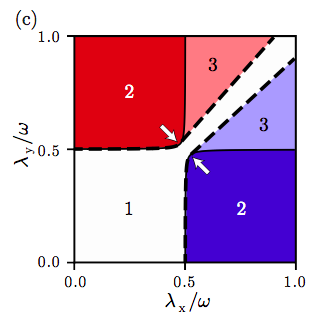
\includegraphics[scale=0.6]{closedsystem}

Transitioning (pun intended) to an open system analysis, we begin with the master equation:
 \begin{equation}
 \frac{d\rho}{d t} = \frac{-i}{\hbar}[H(t),\rho]+\kappa[2a\rho a^{\dagger}-\{a^{\dagger}a,\rho\}]
 \end{equation}

The first term represents standard Hamiltonian evolution, whilst the second represents Markovian cavity dissipation. The paper used a mean-field analysis of to produce a modified phase diagram. The multicritical point violates a requirement on solutions given by spin conservation, so no longer exists and superradiant phases are separated by a new NP sliver. For one coupling strength above criticality and one below, there is the stable existence of one SR solution, while an additional NP solution exists, though is unstable. Stable SR and normal phases coexist for both values of the coupling constant above criticality. For $\omega_{a}=\omega_{c}=\omega$, separation between the two new tricritical points scales linearly with $\kappa$, and so crucially is sensitive to even infinitesimally small cavity dissipation.

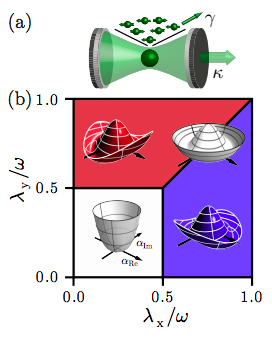
\includegraphics[scale=0.6]{opensystem}

This paper aimed to address the effect of dissipation on the driven-dissipative model featuring a collection of two level atoms interacting with both quadratures of the field of a damped driven optical cavity. I would consider their efforts successful, given the conclusive analysis of the modified open-system phase diagram, characterising new phases and the transitions between them.

Quantum optics is a broad and thriving field of research, from both a theoretical and experimental perspective. It provides an excellent framework to grapple with understanding of ideas underlying quantum 'weirdness', as most models can be implemented experimentally with relative ease. Furthermore it has significant implications for quantum information theory, in particular quantum computing, and thus has the potential for massive practical impact. A major challenge currently facing the field is the experimental implementation of well-studied theoretical models, and developing tools to practically manipulate quibits to store and transmit information, using photons. 
\\
\\1. 	arXiv:1712.09671 [cond-mat.quant-gas]

